\section{多阶段运动中的坐标与事件}
\subsection{先确定所追踪的对象}
综合题的困难常在于一个符号同时指代了不同运动对象。轮心、轮缘物质点、绳切点、杆的几何交点和从动杆端点，可能在某一瞬间位置重合，却有不同的速度和加速度。建模时应先用文字说明所追踪的对象，再为它选坐标；这一说明本身就是列方程的依据。

\fig{k6deep:identity}{原接触物质点离开地面，新的几何接触位置随圆心前进}{\begin{tikzpicture}
\draw[world](-1.5,0)--(3.8,0);\draw[gray,dashed](0,1)circle(1);\draw[world](1.047198,1)circle(1);
\fill(0,0)circle(1.4pt);\draw[guide](0,0)--(-.6,-.5)node[below left]{$P(0)=K(0)$};\fill(.181172,.5)circle(1.6pt)node[left]{$P$};
\fill(1.047198,0)circle(1.5pt)node[below right]{$K$};\fill(1.047198,1)circle(1.2pt)node[right]{$C$};
\draw[guide](1.047198,1)--(.181172,.5);\draw[flow,blue](.181172,.5)--(.581172,1.19282)node[above left]{$\bm v_P$};
\draw[flow,red](1.047198,-.7)--(2.247198,-.7)node[right]{$\dot x_K=U$};\node at(1.2,2.6){实线为转过 $\pi/3$ 后的轮子};
\end{tikzpicture}}
图\ref{k6deep:identity}给同一滚轮上的两个不同追踪对象。$P$ 是开始触地的那个材料标记，随后离开地面；$K=(x_C,0)$ 是每一时刻最下方的几何位置，始终随圆心水平移动。无滑动说的是当下位于 $K$ 的材料点速度为零，并不说坐标函数 $K(t)$ 的导数为零。先确定追踪哪一个对象，才能决定对哪个位置函数求导。

若追踪物质点，可用质点运动方程或刚体速度、加速度关系。若追踪两个曲线的交点，应把两个曲线方程联立，再对交点坐标求导。若研究光滑从动机构，应先列接触法向相对速度为零；只有题设另有无滑动条件时，才增加切向相对速度为零。

\subsection{碰撞时刻连接前后两段}
边界碰撞是事件，不是可以跨越使用同一加速度初值式的普通时刻。光滑固定面上的完全弹性反射，使法向速度反号、切向速度不变。选择沿斜面与法向坐标时，斜面连续反弹的法向运动可周期重复，而切向速度仍被重力分量持续改变。

图\ref{k6t-bounce}中的法向速度在碰撞处跳变，位置连续；每一段抛物线都以该次碰撞后的速度为初值。求“第几次回到起点”，还须要求切向坐标归零的时刻恰为某个碰撞时刻，因而会出现整数条件。只求切向返回时间，可能得到尚在空中的状态。
\fig{k6t-bounce}{弹性反弹的法向速度与连续位置}{\begin{tikzpicture}\draw[axis](0,0)--(6.5,0)node[right]{$t$};\draw[axis](0,-1.6)--(0,1.8)node[above]{$v_n$};\foreach \x in {0,2,4}\draw[world](\x,1.2)--({\x+2},-1.2);\foreach \x in {2,4}\draw[guide](\x,-1.2)--(\x,1.2);\node[below]at(2,-1.3){$T$};\node[below]at(4,-1.3){$2T$};\end{tikzpicture}}

\subsection{测量图像中的不变量}
在斜平面内的抛射，沿等高线方向没有重力分量，对应速度分量恒定。即使图上给的两点不是发射点和落点，也能用这一不变量求时间，再用另一个方向的位移反求加速度。图中横纵格长是否相同必须由标尺确认，不能只按视觉比例量取角度。

\subsection{按事件连接阶段而不是提前指定顺序}
同一题中的落地、绳变松、滑块到杆端和两物体相遇，分别由不同方程定义。可先在当前阶段求出各事件的候选正时间，取其中最早发生的一个作为阶段终点，再以该处状态建立下一阶段。预先指定一个未经检验的碰撞顺序，可能把本来已经落地的轨迹继续延长，或把已经松弛的绳当作定长绳使用。

图\ref{k6t-events-coach}表示位置连续而速度可在碰撞时突变的阶段连接。若阶段从 $t_i$开始，应使用当地时间 $\tau=t-t_i$，把 $\bm r(t_i)$与碰后 $\bm v(t_i^+)$作为初值。连续受力改变时通常速度连续；理想冲量出现时则应使用碰撞规律连接左右速度。每完成一段，都应写清方程的有效区间，再在该区间内筛选根。
\fig{k6t-events-coach}{碰壁处位置连续，速度跳变；碰后用局部时间重新起算}{\begin{tikzpicture}
\begin{scope}
\draw[axis](0,0)--(4.5,0)node[right]{$t$};\draw[axis](0,0)--(0,2.8)node[above]{$x$};
\draw[blue,world](0,0)--(2,2);\draw[red,world](2,2)--(4,0);\draw[guide](2,0)--(2,2)--(0,2);\node[below]at(2,0){$t_1$};\node[left]at(0,2){$x_1$};
\node at(2,3){同一碰撞点连接两段};
\end{scope}
\begin{scope}[xshift=6.1cm]
\draw[axis](0,0)--(4.4,0)node[right]{$t$};\draw[axis](0,-1.6)--(0,2.4)node[above]{$v_x$};
\draw[blue,world](0,1)--(2,1);\draw[red,world](2,-1)--(4,-1);\draw[guide](2,-1)--(2,1);
\node[below right]at(2,0){$t_1$};\node[left]at(0,1){$u$};\node[left]at(0,-1){$-u$};\node at(2,3){碰后 $\tau=t-t_1$};
\end{scope}
\end{tikzpicture}}

\section{刚体机构与约束相容性}
\subsection{同一机构的速度和加速度如何逐杆传递}
对固定长度的杆 $AB$，先以已知端点 $A$为基点写 $\bm v_B=\bm v_A+\omega_{AB}\bm e_z\times\bm r_{B/A}$。若 $B$又属于另一根杆，就有第二个速度表达式。联立两个分量可求未知角速度；此时得到的角速度还不能直接充当常数，因为机构的构形一般继续改变。

再次求加速度时应重新写 $\bm a_B=\bm a_A+\beta_{AB}\bm e_z\times\bm r_{B/A}-\omega_{AB}^2\bm r_{B/A}$，并与另一根杆的表达式联立。驱动匀速只能使驱动杆的角加速度为零，其他杆仍可能有角加速度。每根杆的长度可检验向心项量纲，每个固定铰的加速度应为零，每个共同铰在两侧计算的结果应一致，这三项检查比只核对最终大小更有力。

若速度方程在某构形退化，可能无法由给定输入唯一确定输出，也可能与指定输入矛盾。应保留原分量方程分析其独立性。把一个很小的三角函数放在分母得到很大的输出速度，仅说明机构接近几何奇异；实际能否维持接触、刚性和有限驱动力，还要由题设的理想化条件决定。

\fig{fv:k6:link}{相对速度垂直杆，相对加速度还含沿杆向内的分量}{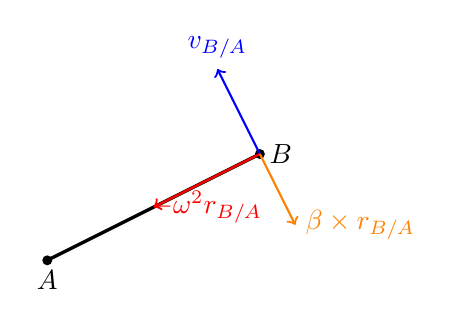
\begin{tikzpicture}[scale=.9]
\coordinate(A)at(0,0);\coordinate(B)at(3,1.5);\draw[very thick](A)--(B);\fill(A)circle(2pt)node[below]{$A$};\fill(B)circle(2pt)node[right]{$B$};
\draw[->,blue,thick](B)--(2.4,2.7)node[above]{$\bm v_{B/A}$};
\draw[->,red,thick](B)--(1.5,.75)node[midway,below]{$-\omega^2\bm r_{B/A}$};
\draw[->,orange,thick](B)--(3.5,.5)node[right]{$\bm\beta\times\bm r_{B/A}$};
\end{tikzpicture}}
图\ref{fv:k6:link}用同一根杆说明速度图不能直接充当加速度图。蓝箭头来自杆长不变，垂直 $AB$；橙箭头来自角速度大小变化；红箭头来自方向变化，始终沿 $BA$。只有将后两项与基点 $A$的加速度相加，才得到 $B$的对地加速度。即使驱动端匀速或某瞬间 $\beta=0$，红色项仍不能删去；机构接近死点时也应回到完整分量方程检查。



\subsection{多接触不一定能全部无滑动}
一个平面圆轮的刚体速度由圆心两个分量和一个角速度确定。两个光滑接触通常给两条法向约束；若再把两处切向滑动都禁止，就可能多出互不相容的条件。遇到两块相向移动的斜面夹轮，须先检查是否存在满足两处完整速度相等的刚体运动。

\fig{k6deep:incompatible}{对称斜面相向挤升时，两个接触点不能同时无滑动}{\begin{tikzpicture}
\draw[world](-2.3,2.3)--(0,0)--(2.3,2.3);\draw[world](0,1.414214)circle(1);
\coordinate(A)at(-.707107,.707107);\coordinate(B)at(.707107,.707107);
\draw[guide](A)--(B);\fill(A)circle(1.4pt)node[left]{$A$};\fill(B)circle(1.4pt)node[right]{$B$};
\draw[flow,blue](A)--++(.5,0)node[above left]{$v$};\draw[flow,red](B)--++(-.5,0)node[below right]{$-v$};
\draw[flow,blue](-2,.2)--(-1,.2);\draw[flow,red](2,.2)--(1,.2);\node at(0,2.9){若均不滑动，接触点将随斜面相向移动};
\end{tikzpicture}}
图\ref{k6deep:incompatible}取两个 $45^\circ$ 斜面、相同速率 $v>0$。两接触点的连线 $AB$ 水平；若都无滑动，轮上两点速度之差为 $(-2v,0)$，也水平。但刚体要求
\[(\bm v_B-\bm v_A)\cdot\overrightarrow{AB}=0,
\]
因为 $AB$ 长度不能改变。图中的假定使这个点积非零，故条件不相容。若允许光滑滑动，只保留两个法向方程，圆心可以竖直上升；滑动正是解除上述矛盾所需的相对运动。

发现无解时，应明确指出哪组约束矛盾，不能悄悄删掉一条后仍称得到“无滑动解”。若改成允许切向滑动的光滑接触，法向方程可单独确定圆心速度，但自转不再仅由几何接触决定。这一对比能区分模型条件与计算技巧。

\subsection{有限滑轮与点滑轮的区别}
忽略滑轮尺寸时，可把直绳段写为圆心之间的距离；保留滑轮半径时，实际绳线沿切线，包角也可能变化。追踪滑轮中心与追踪轮缘点所需信息不同：中心运动可能由绳段变化求出，轮缘点的加速度还需要半径、自转角速度及角加速度。

\fig{k6deep:tangent}{有限半径滑轮的直绳长是切线段长，不是圆心距离}{\begin{tikzpicture}
\draw[world](0,0)circle(1);\coordinate(C)at(0,0);\coordinate(D)at(3,0);\coordinate(T)at(.333333,.942809);\coordinate(S)at(.333333,-.942809);
\draw[world](D)--(T);\draw[world](D)--(S);\draw[guide](C)--(T)node[midway,left]{$b$};\draw[guide](C)--(D)node[midway,below]{$d$};
\fill(C)circle(1.3pt)node[left]{$C$};\fill(D)circle(1.3pt)node[right]{$D$};\fill(T)circle(1.3pt)node[above]{$T$};
\node[above,sloped]at(1.9,.7){$DT=\sqrt{d^2-b^2}$};\node at(1,-1.6){$CT\perp DT$，要求 $d>b$};
\end{tikzpicture}}
图\ref{k6deep:tangent}中，直绳从外点 $D$ 沿切线到达轮缘 $T$，由直角三角形才得到 $DT=\sqrt{d^2-b^2}$。若 $d=d(t)$ 改变而 $b$ 固定，对根式使用链式法则：
\[
\frac{\dd(DT)}{\dd t}
=\frac{1}{2\sqrt{d^2-b^2}}\frac{\dd(d^2-b^2)}{\dd t}
=\frac{2d\dot d}{2\sqrt{d^2-b^2}}
=\frac{d\dot d}{\sqrt{d^2-b^2}}.
\]
切点和包角也随之变化，总绳长还要计入相应圆弧。只有明确采用 $b\to0$ 的点滑轮近似时，才能将这个直段直接替换为 $d$。

对称绳路中，常可直接在两个切点列沿绳速度，避开繁复的弧长微分。题中若出现“某滑轮上下两点”，应先说明它们是顶部、底部的物质点还是即时绳切点；前者用刚体公式，后者还含接触位置变化。不能只凭相同的字母位置把两者互换。

\subsection{解方程后怎样筛选物理分支}
综合题常通过平方、开方、除以三角函数或消去时间来降维。每一步都可能改变解集：平方会失去正负，除式会丢失零分母构形，消去时间会把过去与未来混在同一条曲线上。因此应在推导旁保留 $t>0$、长度正值、角度区间、绳始终绷紧等条件，得到候选根后逐一代回。

例如落体与转杆可能有不止一个空间相交角，最先发生的相遇取最小正的有效时间；若杆有限长，还须检查交点到轴距离。把所有满足无限长直线方程的根都叫碰撞，会忽略杆端边界。对周期反弹，整数碰撞次数是附加条件，也不能由连续时间方程自动保证。

\section{从单条轨迹到一族轨迹}
\subsection{摆线与曲率的局部解释}
匀速滚轮上固定标记的轨迹是摆线。圆心平动与轮缘转动合成后，标记在触地瞬间速度为零，而加速度向上；轨迹在此形成尖点。常规曲率公式要求速率非零，尖点处应讨论两侧极限，不能把公式中零分子、零分母的比值直接当作定义。

求轮缘轨迹时，把初始相位写入三角函数至关重要。初始标记在底部与在顶部，坐标中的正负号不同。图\ref{k6t-cycloid}中，初始位置在地面，转过 $\pi$时到达最高点，转过 $2\pi$时再次触地；这些特殊点可检查坐标式是否正确。
\fig{k6t-cycloid}{摆线的相位和两个触地点}{\begin{tikzpicture}\draw[world](-.3,0)--(7,0);\draw[blue,world]plot[domain=0:360,samples=100]({rad(\x)-sin(\x)},{1-cos(\x)});\foreach \x/\s in {0/0,3.14159/\pi,6.28318/{2\pi}}\node[below]at(\x,0){$\varphi=\s$};\fill(3.14159,2)circle(2pt)node[above]{最高点};\end{tikzpicture}}

\subsection{可达区域与包络线}
对给定初速的一族轨迹，令 $p=\tan\alpha$、$K=gx^2/(2v_0^2)>0$，可把高度直接配方成
\[y=-K\left(p-\frac{x}{2K}\right)^2
+\frac{v_0^2}{2g}-\frac{gx^2}{2v_0^2}.
\]
平方项非正给出所有射法的共同上界，等号给出相切轨迹的方向。若目标低于这个上界，通常有两根；两根还应分别恢复水平速度方向和正的时间。$x=0$时配方所用的 $K$为零，应改用竖直抛射，而不是在中间公式中直接除零。

包络条件解决的是“任一方向能否到达某点”；有障碍时，还要检查整条轨迹是否可行。某个高点在包络内，并不保证通向它的两条轨迹都能越过较近的墙。把局部可达性与全程可行性分开，是从单目标抛射过渡到综合越障题的关键。



\fig{k6deep:obstacle}{目标在包络内，也可能被前方障碍挡住所有命中轨迹}{\begin{tikzpicture}
\draw[axis](0,0)--(3.5,0)node[right]{$x$};\draw[axis](0,0)--(0,2.7)node[above]{$y$};
\draw[gray,dashed,thick]plot[domain=0:3.3,samples=60](\x,{2-(\x)^2/8});
\draw[blue,world]plot[domain=0:2.6,samples=60](\x,{\x-.25*(\x)^2});
\draw[red,world]plot[domain=0:2.35,samples=60](\x,{3*\x-1.25*(\x)^2});
\draw[very thick](.5,0)--(.5,1.4);\fill(2,1)circle(1.5pt)node[right]{$P(2,1)$};\node[above right]at(2.7,1.3){包络};\node[above left]at(.5,1.4){墙顶};
\end{tikzpicture}}
图\ref{k6deep:obstacle}按 $v_0^2/g=4$ 的长度单位绘图。目标 $P(2,1)$ 低于该处包络高度 $3/2$，两条命中轨迹分别有 $\tan\alpha=1,3$。但在墙址 $x=1/2$，它们高度只有 $7/16$ 与 $19/16$，均低于墙高 $7/5$。所以两条数学轨迹都先碰墙，目标虽在自由抛射可达域内，仍不满足这一有障碍问题的全程条件。

另一类可达问题涉及不同运动方式的时间分配，例如先沿岸跑、再游泳。把总时间提出，各段位移变成时间比例乘速度，所有可能的平均速度端点构成凸区域。最远可达方向由边界支持直线确定；既要由投影给出上界，也要给出实际时间比例来证明该上界可实现。

\subsection{时间分配为什么形成凸组合}
设人在两种运动方式中的速度可选为 $\bm u_1,\bm u_2$，分别持续 $t_1,t_2$，总时间 $T=t_1+t_2$。总位移除以 $T$便是 $\overline{\bm u}=\lambda\bm u_1+(1-\lambda)\bm u_2$，其中 $\lambda=t_1/T\in[0,1]$。这不是假设人在全过程匀速，而是把两段实际位移精确相加。追及匀速目标时，双方初始位置若相同，目标速度必须等于这一平均速度。

速度大小有限时，每一种方式的可选速度端点各占一个区域，时间分配产生它们之间的线段。沿目标方向能走多远，应看该射线与所有这些线段所构成区域的边界交点。图\ref{k6t-convex-coach}中，$R$是跑步速度端点，$S$在游泳速度圆上；平均速度 $V$在线段 $RS$上，位置由真实时间占比决定。
\fig{k6t-convex-coach}{两段运动的平均速度在线段上，由时间比例确定}{\begin{tikzpicture}[scale=.9]
\coordinate(O)at(0,0);\coordinate(R)at(4,0);\coordinate(S)at(1,1.732);\coordinate(V)at(2.65,.7794);
\draw[axis](-.3,0)--(4.8,0)node[right]{$V_x$};\draw[axis](0,-.3)--(0,2.7)node[above]{$V_y$};
\draw[world](O)circle(2);\draw[guide](R)--(S);\draw[flow,blue](O)--(R);\draw[flow,red](O)--(S);
\draw[flow](O)--(V);\fill(V)circle(1.6pt)node[above right]{$V$};
\node[below right]at(R){$R$};\node[above]at(S){$S$};\node[below left]at(O){$O$};
\end{tikzpicture}}
求最大可追速度时，还可选一个单位方向 $\bm n$，对所有允许的速度取投影上界。若跑步端点和游泳圆的切点在这一投影上同达上界，它们之间的线段就是边界的一部分。再由目标方向和这条线段的交点求时间比例，才同时完成“不能超过”和“确实达到”两项证明。

\subsection{对称追逐中的尺度与转角}
多个等速物体对称追逐时，构形可保持相似，整体大小缩小同时绕中心转动。应把速度分成径向缩小与切向转动两部分：前者确定相遇时间，后者决定轨迹形状。距离趋零时角速度可能发散，因此有限时间相遇与绕中心无限多圈并不矛盾，关键在于每圈的尺度也趋零。
\subsection{对称性必须能在演化中保持}
对称追逐不能只凭初始图形便宣称各时刻仍相似。应说明运动规则在旋转和重新编号后不变，且每个时刻都按同一规则朝下一物体运动，于是三条运动方程彼此由对称变换对应。由运动解的局部唯一性，在尚未相遇的区间，等边构形持续保持，中心也保持固定；这才允许用一个边长和一个转角描述全部运动。

\fig{k6deep:pursuit}{等边追逐的速度同时缩小半径并转动构形}{\begin{tikzpicture}
\coordinate(A)at(2,0);\coordinate(B)at(-1,1.732051);\coordinate(C)at(-1,-1.732051);
\draw[world](A)--(B)--(C)--cycle;\draw[guide](0,0)--(A);\fill(0,0)circle(1.4pt)node[below]{$O$};
\foreach \n in {A,B,C}{\fill(\n)circle(1.4pt);}\node[right]at(A){$A$};\node[above]at(B){$B$};\node[below]at(C){$C$};
\draw[flow,blue](A)--(.96077,.6)node[above right]{$\bm u$};\draw[flow,red](A)--(.96077,0)node[midway,below]{$-\sqrt3u/2$};
\draw[flow,green!50!black](.96077,0)--(.96077,.6)node[left]{$u/2$};\node at(.5,-2.4){沿 $AB$ 的速度相对 $AO$ 偏转 $30^\circ$};
\end{tikzpicture}}
在图\ref{k6deep:pursuit}的顶点 $A$，速度沿边 $AB$，向心投影为 $u\cos30^\circ=\sqrt3u/2$，切向投影为 $u\sin30^\circ=u/2$。因此
\[\dot\rho=-\frac{\sqrt3u}{2},\qquad \rho\dot\varphi=\frac u2.
\]
第一式直接决定何时到中心，第二式决定图形怎样旋转。不能把全部速率 $u$ 当作向心速度，否则相遇时间会偏小，也无法解释弯曲的追逐轨迹。

若径向缩小速度为常量，半径会在有限时间趋零；切向速度有限时角速度却是切向速度除以半径，可随之发散。指定 $\rho(0)=\rho_0$、$\varphi(0)=\varphi_0$。先从径向方程积分：
\[
\rho(t)-\rho_0
=-\frac{\sqrt3u}{2}\int_0^t\dd s
=-\frac{\sqrt3u}{2}[s]_0^t
=-\frac{\sqrt3u}{2}t.
\]
因此 $\rho=\rho_0(1-t/T)$，其中到达中心的时间为
$T=2\rho_0/(\sqrt3u)$。再把两个微分方程相除，消去时间：
\[
\frac{\dd\rho}{\dd\varphi}
=\frac{-\sqrt3u/2}{u/(2\rho)}=-\sqrt3\rho.
\]
相遇前 $\rho>0$，可分离变量并保留初值：
\[
\int_{\rho_0}^{\rho}\frac{\dd s}{s}
=-\sqrt3\int_{\varphi_0}^{\varphi}\dd\psi,\qquad
[\ln s]_{\rho_0}^{\rho}
=-\sqrt3[\psi]_{\varphi_0}^{\varphi}.
\]
所以 $\ln(\rho/\rho_0)=-\sqrt3(\varphi-\varphi_0)$，即
$\rho=\rho_0e^{-\sqrt3(\varphi-\varphi_0)}$。这是形状方程；把径向解代回则得
$\varphi-\varphi_0=-(1/\sqrt3)\ln(1-t/T)$，仅在 $0\le t<T$ 使用。把有限路程、无限转角与有限时间联系起来，能够检查最终结论是否把角速度与线速度混淆。

\subsection{上界证明与实现方案相配合}
求最大可追船速时，某个方向上的投影不等式能给出速度上界，但尚不能证明该值可行。必须找出跑步与游泳时间比例，使水平、竖直两分量同时满足追及关系。反过来，给出一个成功方案只能证明至少能达到该速度，若没有全体方案的上界，就不能称为最大值。

包络、速度圆切线和均值不等式都是把这两步连接起来的方法：等号条件给出实现方案，边界不等式给出全局限制。写解答时应明确哪一步说明“任何方案都不能超过”，哪一步说明“这个方案确实达到”，而不只说“由对称性可知最优”。

\subsection{用特殊点检查图与解析式}
摆线可检查两触地点和最高点，机构可检查对称位置与死点，绳路可检查水平和竖直极限，追逐可检查相遇时边长归零。图中的速度箭头应与解析分量一致，加速度箭头须按所选时刻的符号绘制，不能只画一个随意朝向的合箭头。

图形还承载适用条件：斜面接触点要真正落在圆周与斜线上，转杆交点要在杆长内，反弹墙址要处于对应的运动段，有限半径滑轮的绳应沿切线。把代数根代回图中的位置关系，可以检查它是否落在实际杆段、绳段和运动区间内。几何边界与时间边界都满足，才构成完整的可行解。

